

\documentclass[a4paper]{article}

\usepackage{amsmath}
\usepackage{hyperref}
\usepackage{biblatex}
\usepackage{enumerate}
\usepackage{graphicx}
\usepackage{stmaryrd}
\usepackage[dvipsnames]{xcolor}
\usepackage{listings}
\usepackage{caption}
\usepackage{subcaption}
\usepackage{booktabs}


\addbibresource{refs.bib}

\begin{document}

\author{Ola Bratt \\
  \href{mailto:ola.bratt@gmail.com}{ola.bratt@gmail.com}
  \and
  Patrick Attimont \\
  \href{patrickattimont@gmail.com}{patrickattimont@gmail.com}
}

\title{DAT565/DIT407 Assignment 2}
\date{2024-01-xx}

\maketitle

This paper is addressing the assignment 2 study queries within the \emph{Introduction to Data Science \& AI} course, DIT407 at 
the University of Gothenburg and DAT565 at Chalmers. The main source of information for this project
is derived from the lectures and Skiena~\cite{Skiena:2024}. 
\section*{Problem 1: Scrapping house prices}
Problem 1 have been solved using BeautifulSoup together with simple string operations such as 
\begin{verbatim}
  split, replace and strip, 
\end{verbatim}
also regaular expressions have been used to idefity certain information. The code can be found in the appendix.

\section*{Problem 2: Analyzing 2022 house sales}
To caluculate the five-number summary of the closing prices of the houses prices we simply used 
\begin{verbatim}
describe()
\end{verbatim}
on the dataframe containing the closing prices. The result can be seen in table~\ref{tabular:five_number_summary}.\\

When generating the histogram depicting closing prices (see Figure~\ref{fig:histogram_closing_price}), we employed the "square root method" to determine the bin size. This method was chosen for its ability to unveil trends while maintaining a balance, as larger bins would obscure relevant features, such as the dip around 4.000.000 kr. The resulting plot exhibits a right skew, which is expected given the scarcity of high-priced houses.

Figure~\ref{fig:closing_price_house_ares} displays the relationship between closing prices and house areas, while Figure~\ref{fig:closing_price_house_ares_color} illustrates the same relationship, with the number of rooms colorized.


\begin{table}
  \begin{center}
  \begin{tabular}{c c}
    min & 250000 \\
    \text{25\%} & 3200000 \\
    \text{50\%} & 4100000 \\
    \text{75\%} & 5035000 \\
    max & 21000000 \\
  \end{tabular}
\end{center}
\caption{Five-number summary of closing prices}
  \label{tabular:five_number_summary}
\end{table}

\newpage

\begin{figure}
  \centering
  \begin{subfigure}[a]{\textwidth}
      \centering
      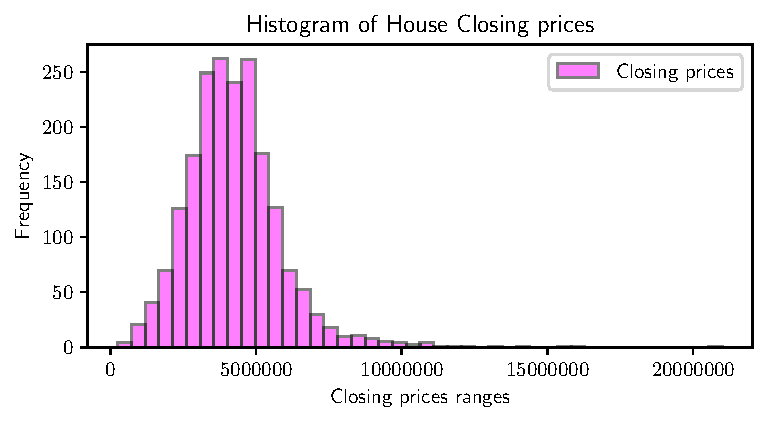
\includegraphics[width=\textwidth]{histogram_closing_price.pdf}
      \caption{Closing prices of houses}
      \label{fig:histogram_closing_price}
  \end{subfigure}
  \vfill
  \begin{subfigure}[b]{\textwidth}
      \centering
      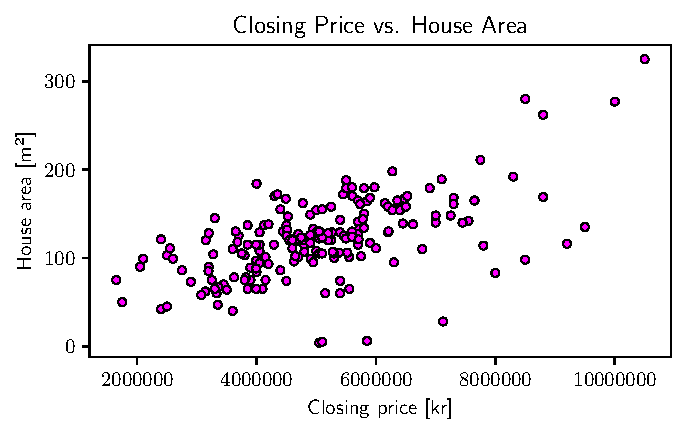
\includegraphics[width=\textwidth]{closing_price_house_ares.pdf}
      \caption{Closing price vs house area}
      \label{fig:closing_price_house_ares}
  \end{subfigure}
  \vfill
  \begin{subfigure}[c]{\textwidth}
      \centering
      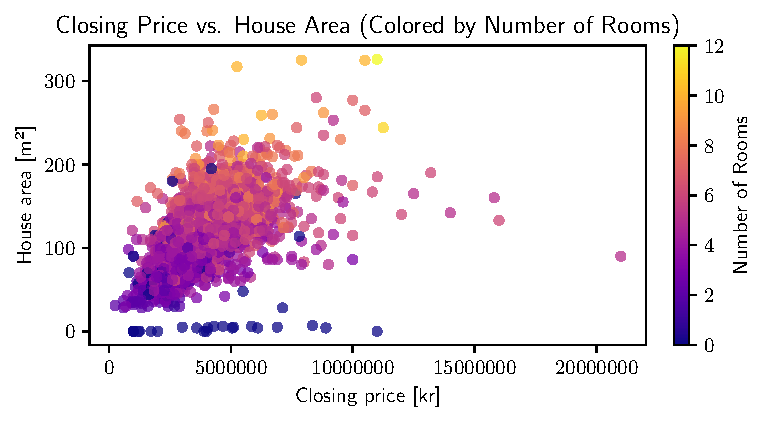
\includegraphics[width=\textwidth]{closing_price_house_ares_color.pdf}
      \caption{Closing price vs house area with color}
      \label{fig:closing_price_house_ares_color}
  \end{subfigure}
     \caption{Plots of house prices}
     \label{fig:house_plots}
\end{figure}


\newpage

\section*{Discussion}

\newpage


\printbibliography

\section*{Appendix: Source Code}

\lstset{
  language=Python,
  basicstyle=\ttfamily,
  commentstyle=\color{OliveGreen},
  keywordstyle=\bfseries\color{Magenta},
  stringstyle=\color{YellowOrange},
  numbers=left,
  basicstyle=\footnotesize,
  breaklines=true,
  postbreak=\mbox{\textcolor{red}{$\hookrightarrow$}\space}
}


\lstinputlisting{ola/assignment2.py}

\end{document}
